%\documentclass[11pt]{scrartcl}
\documentclass[11pt, twoside, a4paper, BCOR8mm, DIV12, bibtotoc,idxtotoc]{scrbook}
\usepackage{german}
\usepackage{typearea}
\usepackage{longtable}
\usepackage{hyperref}
\usepackage{graphicx}

% Zusaetzliche Picture-Umgebungen (z.B. shadowenv)
\usepackage{picins}

% Header anpassbar
\usepackage{fancyhdr}

% Headings umdefinieren
\pagestyle{fancy}
\fancyhf{}
\fancyhead[RO]{\nouppercase{\rightmark}}
\fancyhead[LE]{\nouppercase{\leftmark}}
\fancyfoot[RO, LE]{\thepage}

%\addtolength{\headwidth}{\marginparsep}
%\addtolength{\headwidth}{\marginparwidth}
\addtolength{\headwidth}{1cm}

\parindent0.0mm
\parskip0.3cm    
\typearea{13}

\begin{document}

\frontmatter

\begin{titlepage}

\begin{center}
\rule[-.1in]{16cm}{1mm}\\[3mm]
{\fontfamily{cmss}\fontseries{bx}\fontshape{n}\fontsize{20}{20pt}\selectfont
  www.openbib.org $\bullet$ OpenBib Rechercheportal}\\[-2mm]
\rule[-.1in]{16cm}{1mm}

\vspace{5cm}

  \textbf{\fontfamily{cmss}\fontseries{bx}\fontshape{n}\fontsize{30}{30pt}\selectfont OpenBib Recherche-Portal\\[3mm] Technische Dokumentation}

  \vspace{2cm}

  Oliver Flimm \texttt{<flimm@openbib.de>}\\
  Stand: \today

  \vspace{8cm}

\rule[-.1in]{16cm}{1mm}\\[3mm]
{\fontfamily{cmss}\fontseries{bx}\fontshape{n}\fontsize{20}{20pt}\selectfont
  www.openbib.org $\bullet$ OpenBib Rechercheportal}\\[-2mm]
\rule[-.1in]{16cm}{1mm}

\end{center}

\end{titlepage}

%\thispagestyle{empty}

%\begin{verbatim}


%Copyright (c) 2004 Oliver Flimm <flimm@openbib.org>

%Es wird die Erlaubnis gegeben dieses Dokument zu kopieren, verteilen 
%und/oder zu veraendern unter den Bedingungen der GNU Free
%Documentation License, Version 1.1 oder einer spaeteren, von der Free 
%Software Foundation veroeffentlichten Version; mit den
%Unveraenderlichen Abschnitten DEREN TITEL AUFGEZAEHLT sind, mit den 
%Vorderseitentexten die AUFGEZAEHLT sind, und mit den Rueckseitentexten
%die AUFGEZAEHLT sind. Eine Kopie dieser Lizenz ist in dem Abschnitt 
%enthalten, der mit "GNU Free Documentation License"
%\end{verbatim}

\tableofcontents

\mainmatter

\chapter{Generelle Architektur}

Die OpenBib-Portalsoftware-Suite ist in logischen Schichten
organisiert. Ein Schaubild der ge\-ne\-rellen Architektur zeigt Abb.
\ref{bild:architektur}. Dieses Kapitel soll einen kurzen Abri"s dieser
Architektur geben, damit die gr"o"seren Zusammenh"ange deutlich
werden. Die Schichten von 'unten' nach 'oben' sind: Die
datenbankabh"angige Schicht, die datenbank"ubergreifende Schicht, die
Portal-Schicht mit weiteren externen Zugriffsmechanismen (DigiBib,
UK-Online) und schlie"slich die Lastverteilungs-Schicht. Diese
Schichten werden bei der Interaktion mit einem Benutzer bei der
Verwendung des OpenBib-Portals in entgegengesetzter Richtung von
'oben' nach 'unten' durchlaufen.


\begin{figure}
\begin{shadowenv}
  \vspace{4mm}
    \centering \begin{minipage}[b]{1.0\textwidth}
      \centering 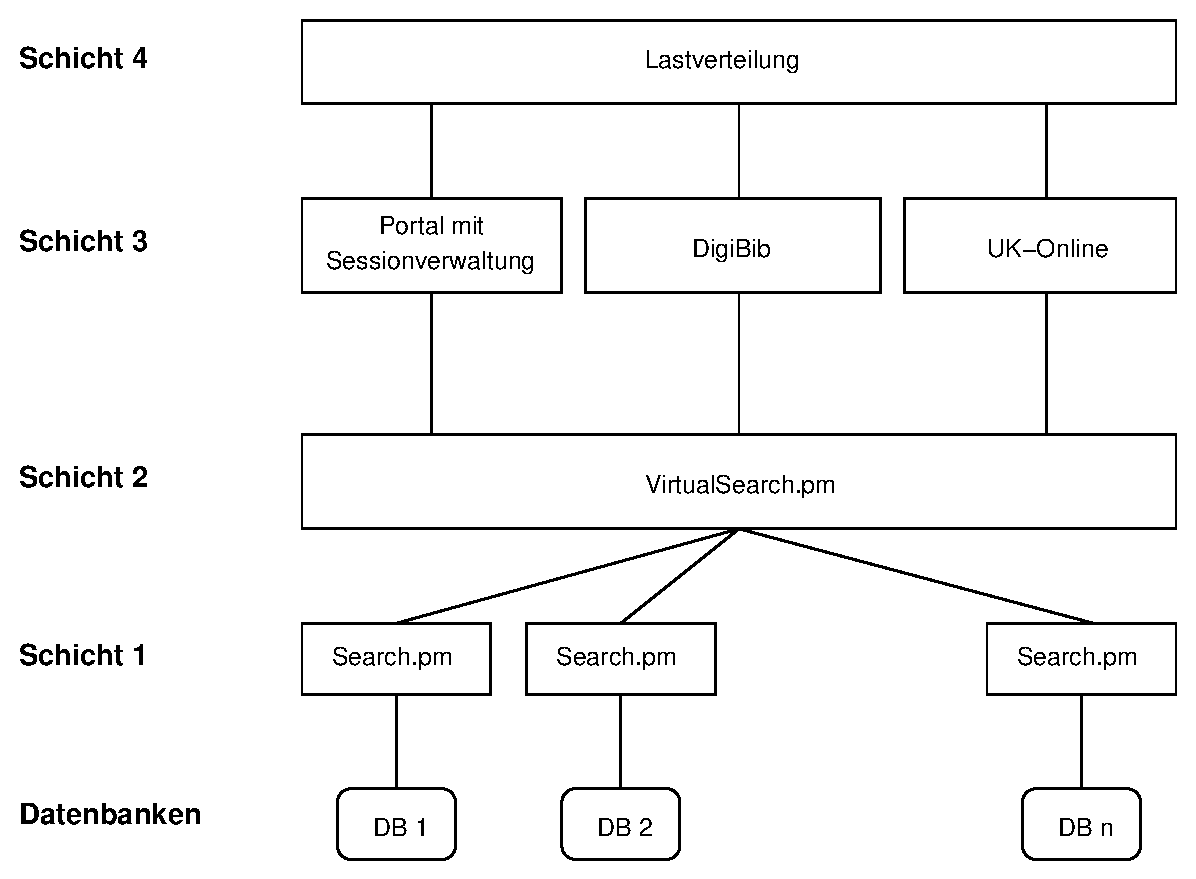
\includegraphics[width=12cm]{schicht04.eps}
    \end{minipage}
    \caption{Generelle Architektur der OpenBib-Portal-Suite}
  \label{bild:architektur}
  \vspace{3mm}
\end{shadowenv}
\end{figure}

\section{Die datenbankabh"angige Schicht 1 -- \texttt{OpenBib::Search}}

In der untersten, der datenbankabh"angigen Schicht greift das Perl-Modul
\texttt{OpenBib::Search} auf eine feste Datenbank zu. Welche
Datenbank dies ist, kann als Aufrufparamter dem Programm mitgegeben
werden. Dadurch ist es m"oglich, das gleiche Programm f"ur Recherchen
"uber ver\-schie\-de\-ne Daten\-banken zu nutzen. Das Modul selbst -- wie
auch alle anderen unter \texttt{openbib/portal} angesiedelten -- ist als
Erweiterung des Apache-Webservers via \texttt{mod\_perl} realisiert.
Dadurch arbeitet es au"ser\-ordentlich schnell.


\section{Die datenbank"ubergreifende Recherche-Schicht 2 -- \texttt{OpenBib::VirtualSearch}}

Die datenbank"ubergreifende Recherche geschieht in der "uber
\texttt{OpenBib::Search} liegenden Schicht 2 (vgl. Abb.
\ref{bild:architektur}) mit dem Perl-Modul
\texttt{OpenBib::VirtualSearch}. Aufgabe dieses Programms ist es,
eine Suchanfrage und eine Anzahl an Recherche-Datenbanken vom Benutzer
entgegen\-zuneh\-men und genau diese eine Suchanfrage sequentiell an das
Modul \texttt{OpenBib::Search} f"ur jede der "ubergebenen
Datenbanken zu schicken. 

Die Ergebnisse der einzelnen Recherchen werden entgegengenommen und in
Listenform auf\-be\-rei\-tet. Die jeweiligen Titel selbst sind in dieser
Gesamttrefferliste via URL mit einer Suchanfrage f"ur genau diesen
Einzeltreffer mit \texttt{OpenBib::Search} verkn"upft. 
Bei der
Auswahl eines einzelnen Treffers wird dadurch direkt in die
zugeh"orige Datenbank via \texttt{OpenBib::Search} gesprungen. 

Alle 'normalen' Verkn"upfungs-Links (Normdaten, Hierarchien, etc.)
beziehen sich -- wir befinden uns nach der Auswahl eines Treffer wieder in
Schicht 1 -- auf genau diese eine Datenbank. "Uber das gro"se
stilisierte 'G' bei den Normdaten kann jedoch auch an dieser Stelle
wieder eine datenbank"ubergreifende Recherche nach genau dem
zugeh"origen Begriff gestartet werden. Der Benutzer hat somit bei
einem Einzeltreffer immer die Moeglichkeit selbst zu entscheiden, ob
er sich bzgl. der Normdaten weiter im zugeh"origen Katalog aufhalten
m"ochte, oder katalog"ubergreifend Recherchieren m"ochte.

Da in jedem Katalog die Verkn"upfungen bereits in der Datenbank
existieren, ist ein 'sich treiben lassen' in einem festen Katalog
au"ser\-ordentlich schnell, w"ahrend bei einer katalog"ubergreifenden
Suche ein kleiner Tribut zu zahlen ist, da nun alle Datenbanken mit
einer 'neuen Suche' abgefragt werden.

Da \texttt{OpenBib::VirtualSearch} letztlich f"ur die
datenbank"ubergreifende Gewinnung der Recherche\-er\-geb\-nisse zust"andig
ist, werden nach erfolgreicher Recherche die Ergebnisse aufgeteilt
nach den einzelnen Katalogen in der Session-Datenbank \texttt{session}
'gecached'. Durch das Caching der Re\-cher\-che\-ergebnisse kann von
\texttt{OpenBib::VirtualSearch} auch eine Trefferlistenfunktionalit"at
geleistet werden, in der man "uber die Ergebnisse der letzten
Recherche hinaus auch noch direkt auf die Ergebnisse jeder zuvor eingegebenen
Suche in der aktuellen Session zugreifen kann.

\section{Die Portal-Schicht 3 mit ihren externen Zugriffmechanismen}

\subsection{Das Portal mit Session- und Benutzerverwaltung}

In der Portalschicht wird dem Benutzer sessionbasiert in einer aus
zwei Frames bestehenden Web-Seite eine Arbeits- und Recherche-Oberfl"ache
geliefert. 

Der Einsprung-URL in das Portal wird durch das Modul
\texttt{OpenBib::StartOpac} realisiert.

Das Modul \texttt{OpenBib::StartOpac} kann "uber verschiedene Parameter
gesteuert werden, die z.B. f"ur den direkten Sprung zu einem Treffer
einer Datenbank oder der Anzeige einer katalogeigenen Sicht des
Portals Verwendung finden und gegebenenfalls an nachgelagerte Module
durchgereicht werden. Seine wesentliche Aufgabe ist jedoch, eine
eindeutige Session-ID zu generieren sowie ein Frameset mit zwei Frames
bereitzustellen.  Das obere Frame f"ur die Navigation wird durch das Modul
\texttt{OpenBib::HeaderFrame} gef"ullt, das untere Frame standardm"a"sig
zuerst durch das Modul \texttt{OpenBib::SearchFrame}, das dem
Navigations-Element 'Recherche' entspricht.

Das Modul \texttt{OpenBib::HeaderFrame} ist f"ur die Navigation im Portal
inklusive Counter f"ur die Merkliste zust"andig.

In der Navigation werden folgende Funktionalit"aten angeboten:

\begin{description}
\item[Kataloge] Die Auswahl der zu durchsuchenden Kataloge geschieht
  "uber eine entsprechende Aus\-wahl\-seite, die durch das Modul
  \texttt{OpenBib::DatabaseChoice} generiert wird.
\item[Recherche] Die Recherche-Maske wird "uber einen Aufruf von
  \texttt{OpenBib::SearchFrame} dargestellt.
\item[Trefferliste] Ein Zugriff auf Trefferlisten aus vorangegangenen
  Recherchen geschieht "uber das Modul \texttt{OpenBib::VirtualSearch},
  welches neben der verteilten Recherche auch f"ur ein Caching der
  Ergebnis-Daten zust"andig ist.
\item[Merkliste] Die Anzeige, Organisation sowie der Mailversand der
  Merkliste wird durch die Module
  \texttt{OpenBib::ManageCollection} und \texttt{OpenBib::MailCollection}
  "uber\-nom\-men. Bei Auswahl eines Treffers f"ur die Merkliste wird
  \texttt{OpenBib::HeaderFrame} aktualisiert, und zeigt die neue Zahl
  gemerkter Treffer an.
\item[Login / Benutzereinstellungen] "Uber das Modul \texttt{OpenBib::Login}
  kann sich der Benutzer am Portal authentifizieren und so von
  weiteren personalisierten Funktionalit"aten profitieren. Dazu
  geh"oren neben generellen Benutzereinstellungen
  (\texttt{OpenBib::UserPrefs}) u.a. per\-sis\-ten\-te Merklisten sowie
  Datenbankprofile (\texttt{OpenBib::DatabaseProfile}).

  Das Modul gew"ahrt dabei den Zugang auf Grundlage seiner eigenen
  Datenbank, die "uber das Modul \texttt{OpenBib::SelfReg} via
  Selbstregistierung gef"ullt wird, bzw. von Fremddatenbanken des
  Bibliothekssystems Sisis SunRise "uber die SLNP-Schnittstelle der
  gleichnamigen Firma. Falls ein Benutzer sein selbstregistriertes
  Passwort vergessen hat, so kann er es sich "uber das Modul
  \texttt{OpenBib::MailPassword} per Mail zusenden lassen.
\item[Hilfe] Die Hilfeseite wird direkt als URL
  \texttt{/suchhilfe.html} angesprochen
\item[Sitzung beenden] Beim Ende der Sitzung wird zum Modul
  \texttt{OpenBib::Leave} gesprungen, welches die sessionrelevanten Daten
  entfernt sowie einen URL in die Schicht 4 zur Lastver\-teilungs\-instanz
  \texttt{OpenBib::LoadBalancer} mit Angabe eines eventuell aktiven Views
  (Institutssicht) f"ur einen er\-neu\-ten Einstieg in das Such-Portal
  bereitstellt.

\end{description}

\subsection{Externe Anbindung an die DigiBib}

Neben der Bereitstellung einer Recherche- und Arbeitsoberfl"ache f"ur
den Endbenutzer, besteht auch die M"oglichkeit automatisiert auf den
Gesamtkatalog zuzugreifen.

Eine solche M"oglichkeit besteht in der Einbindung in das Such-Portal
\textbf{Digitale Bibliothek NRW} (DigiBib) des
Hoch\-schul\-bibliotheks\-zentrum NRW. Das Suchinterface besteht aus
einem fest definierten Such-URL und einem fest definierten
HTML-basierten Antwortformat f"ur die Treffer. Grunds"atzlich wird auf
eine Rechercheanfrage, z.B. unter Angabe eines Suchbegriffes f"ur den
Titel, mit einer Kurztitelliste geantwortet. Es kann bestimmt werden,
welcher Teil der Kurztitelliste von den OpenBib-Daten\-banken
angefordert werden darf (Bl"atterfunktion mit frei w"ahlbarem Offset
und Schrittweite). Dar"uberhinaus wird neben der Kurztitelliste auch
die Anzeige eines Einzeltreffers mit weiter\-gehen\-den Kategorien
angeboten. In der Kurztitelliste sind alle Informationen vorhanden, um
den Einzeltreffer aufzurufen.

\subsection{Externe Anbindung an UK-Online}

Eine weitere Anbindung besteht in das Universit"atsportal UK-Online
von Herrn Dr. Lohnstein aus der Philosophischen Fakult"at der
Universit"at zu K"oln. Hier wird in UK-Online die M"oglichkeit
angeboten eigenen Bibliographie-Listen zu verwalten. Der Aufbau einer
solchen Bibliographie-Liste geschieht "uber die Recherche in OpenBib
und anschlie"sende Umwandlung und Ab\-spei\-cherung in ein
Bibliographie-Listen-Format.

Nach dem derzeitigen Stand sind beide externen Anbindung noch nicht in
einer lastverteilten Variante verf"ugbar. Diese ist jedoch kurz vor
der Fertigstellung.

\section{Die Lastverteilungs-Schicht 4}

Die Lastverteilungs-Schicht ist der erste Anlaufpunkt f"ur die
Benutzung von OpenBib. Diese Schicht wird f"ur das Portal durch das
Modul \texttt{OpenBib::LoadBalancer} und \texttt{OpenBib::ServerLoad} gebildet.
Entscheidungsgrundlage f"ur die Verteilung ist die Auslastung der
betroffenen Recher bzw. deren generelle Ansprechbarkeit.

Durch diese vorgeschaltete Verteilung der Recherche-Sitzungen auf
mehrere Rechner ergeben sich mehrere Vorteile:

\begin{enumerate}
\item Es wird eine Lastverteilung durchgef"uhrt. Wenn also ein Nutzer
  einen dieser URL's aufruft, so wird er auf den Rechner
  weitergeleitet, der am wenigsten zu tun hat.  Dies ist prim"arer
  Zweck dieser Schicht.
\item Ist ein Rechner defekt (im Sinne von tot), dann wird er bei der
  Verteilung/Weiterleitung nicht mehr ber"ucksichtigt und die Benutzer
  werden nur noch auf die verbliebenen Rechner verteilt. In diesem
  Fall ist bei der Weiterleitung mit einer kurzen Wartezeit von
  maximal 5 Sekunden (Timeout) zu rechnen.  Automatisch wird
  zus"atzlich an den Administrator eine Mail ge\-ne\-riert, die ihn
  auf den defekten Rechner hinweist. Ein Sonderfall ist natuerlich der
  'Verteilungs\-rech\-ner' selbst, bei dessen Ableben tempor"ar ein
  anderer Rechner unter seiner Identitaet einspringen mu"s. Letzteres
  kann selbstverst"andlich nicht automatisch geschehen und muss
  manuell konfiguriert werden.
\item Werden Wartungsarbeiten auf einem der Rechner ausgef"uhrt, so
  kann man ihn selbst tempor"ar aus der Verteilung/Weiterleitung
  herausnehmen. Auf diese Weise "andert sich f"ur die Nutzer nichts,
  es werden dann die verbliebenen Rechner verwendet.
\end{enumerate}

\appendix

\chapter{Tabellen in \texttt{session.mysql}}

In diesem Anhang werden die einzelnen Tabellen in der
Session-Datenbank beschrieben.

\begin{description}
\item[session] Dies ist die prim"are Tabelle in der die
  \texttt{sessionid} f"ur eine Nutzersitzung abgespeichert wird.
  Zus"atzlich wird die Anfangszeit der Session \texttt{createtime}
  gespeichert. 
\item[treffer] Diese Tabelle realisiert sessionabh"angig die
  \textbf{Merkliste}. Es werden zu jeder Session der Datenbankname sowie die
  Identifikations-Nr des gemerkten Titels abgespeichert.
\item[sessionlog] Diese Tabelle soll im Betrieb mit relevanten
  Informationen gef"ullt werden, die dann statistisch ausgewertet
  werden k"onnen. Derzeit wird sie nicht verwendet.
\item[queries] In dieser Tabelle werden sessionabh"angig die
  Suchanfragen inkl. gefundener Treffer ab\-ge\-spei\-chert. Dadurch ist es
  m"oglich sich "altere Suchanfragen wieder in die Recherchemaske
  eintragen zu lassen.
\item[dbchoice] In dieser Tabelle wird die vom Benutzer vorgenommene
  Datenbankauswahl session\-ab\-h"angig abgespeichert.
\item[dbinfo] In dieser Tabelle werden Informationen zu den einzelnen
  Katalogdatenbanken ab\-ge\-spei\-chert. Dazu geh"ort die Fakult"at
  (\texttt{faculty}, derzeit fest in den Modulen einprogrammiert),
  eine Beschreibung (\texttt{description}), das Katalogisierungssystem
  (\texttt{system} anhand K"urzel), der Datenbankname
  (\texttt{dbname}), das Bibliothekssigel (\texttt{sigel}) und
  schlie"slich die wesentliche Information, ob die Datenbank im Portal
  aktiv ist oder nicht (\texttt{active}). "Uber die letzte Einstellung
  lassen sich im laufenden Betrieb Datenbanken ein- und ausblenden.
\item[dboptions] Zu jeder Datenbank werden hier Informationen
  abgelegt, wo die zum Aufbau der Datenbank notwendigen Daten liegen
  und alle zum Heranschaffen der Daten ben"otigten Informationen wie
  Rechnername (\texttt{host}), Pfade, Dateinamen, Zugriffsprotokoll
  (\texttt{lokal}, \texttt{http}, \texttt{ftp}) und
  Authentifizierungsinformationen wie Benutzernamen oder Passworte.
  Derzeit sind diese Informationen schon im Wesentlichen vorhanden,
  sie werden durch die automatischen Konvertierungsskripte jedoch noch
  nicht verwendet.
\item[titcount] In dieser Tabelle wird die Anzahl der Titel pro
  Datenbank festgehalten. Diese Information wird "uber das Modul
  \texttt{OpenBib::SearchFrame} f"ur den Benutzer ausgegeben. Das Setzen
  dieser Werte geschieht "uber die automatischen
  Konvertierungsskripte.
\item[searchresults] In dieser Tabelle wird session\-ab\-h"an\-gig zu jeder
  Suchanfrage (\texttt{queryid} der \texttt{queries}-Tabelle) pro
  Datenbank das Ergebnis gecached. Zus"atzlich wird jeweils auch noch
  die Anzahl der Treffer in der jeweiligen Datenbank
  ab\-ge\-spei\-chert. Durch diese Tabelle in Verbindung mit der Tabelle
  \texttt{queries} wird die \textbf{Trefferliste} realisiert.

\item[viewinfo] In dieser Tabelle werden zu einer Recherche-Sicht
  (view) neben dem den View de\-fi\-nier\-enden Viewnamen
  (\texttt{viewname}) auch eine Beschreibung \texttt{description}
  abgelegt. Die Informatione, ob der View aktiv ist oder nicht
  (\texttt{active}) wird derzeit nicht genutzt.
\item[viewdbs] In dieser Tabelle werden zu dem Viewnamen die Datenbanken
  festgelegt, die mit der konkreten Recherche-Sicht assoziiert
  sind. Hier k"onnen auch mehrere Datenbanken ein\-ge\-tra\-gen werden.
\item[sessionview] "Uber diese Tabelle wird die Nutzung eines Views
  durch eine Session festgehalten. Diese Information wird ben"otigt,
  damit im oberen Frame (\texttt{OpenBib::HeaderFrame}) wie auch in der
  Recherchemaske (\texttt{OpenBib::SearchFrame}) die View-Informationen
  zus"atzlich angezeigt werden. Derzeit wird in \texttt{OpenBib::HeaderFrame}
  auf ein Bild mit dem Namen des Views 

\begin{verbatim}
HTDOCS/images/kvik/views/<viewname>.png
\end{verbatim}

  verwiesen sowie in \texttt{OpenBib::SearchFrame} ein fester Satz unter
  Einbeziehung der Be\-schrei\-bung des Views ausgegeben.

\end{description}

\chapter{Tabellen in \texttt{pool.mysql}}

Die Tabellen in \texttt{pool.mysql} werden nach Norm- bzw.
Stamm-Dateien geordnet dargestellt. Es sind dies \emph{Titel},
\emph{Verfasser}, \emph{K"orperschaften}, \emph{Notationen},
\emph{Schlagworte} sowie \emph{Exemplardaten} und
\emph{Bibliotheksdaten}. Dar"uberhinaus gibt es eine zus"atzliche
Tabelle \texttt{search} in der in Form einer Volltextsuche
recherchiert werden kann. Verkn"upfungen zwischen den Norm-Dateien
sind bereits durch entsprechende Verkn"upfungstabellen in der
Datenbank abgebildet.


\section{Titel-Normdaten}

\subsection{Einfache Kategorien}

\begin{description}
\item[tit] In dieser Tabelle befinden sich Titelinformationen, die
  nicht mehrfach vorkommen. "Uber die Spalte \texttt{idn} k"onnen
  Verkn"upfungen zu multiplen Kategorien in anderen Tabellen
  hergestellt werden. Ebenso k"onnen durch Kopplungstabellen damit
  Verkn"upfungen zwischen Titeln realisiert werden.
\item[titpsthst] Enth"alt die multiple Kategorie \textbf{PST/HST} .
\item[titgtunv] Enth"alt die multiple Kategorie \textbf{GT unverkn}.
\item[titisbn] Enth"alt die mutliple Kategorie \textbf{ISBN}
\item[titissn] Enh"alt die multiple Kategorie \textbf{ISSN}.
\item[titner] Enth"alt die multiple Kategorie \textbf{NE/R}.
\item[titteiluw] Enth"alt die multiple Kategorie \textbf{Teil UW}.
\item[titstichw] Enth"alt die multiple Kategorie \textbf{Stichwort}.
\item[titwst] Enth"alt die mutliple Kategorie \textbf{WST}.
\item[titurl] Enth"alt die multiple Kategorie \textbf{URL}.
\item[titnr] Enth"alt die multiple Kategorie \textbf{NR}.
\item[titartinh] Enth"alt die multiple Kategorie \textbf{Art/Inhalt}.
\item[titphysform] Enth"alt die multiple Kategorie
  \textbf{Physikal. Form}.
\end{description}


\subsection{Verkn"upfungs-Kategorien}

\begin{description}
\item[titgtm] Verkn"upfung zwischen Titeln "uber die Kategorie
  \textbf{GTM}.
\item[titgtf] Verkn"upfung zwischen Titeln "uber die Kategorie
  \textbf{GTF}.
\item[titinverkn] Verkn"upfung zwischen Titeln "uber die Kategorie
  \textbf{IN verkn.}.
\item[titswtlok] Verkn"upfung zu den Schlagwort-Normdaten "uber die
  Kategorie \textbf{SWT lokal}.
\item[titswtreg] Verkn"upfung zu den Schlagwort-Normdaten "uber die
  Kategorie \textbf{SWT reg}.
\item[titverf] Verkn"upfung zu den Verfasser-Normdaten "uber die
  Kategorie \textbf{Verfasser}.
\item[titpers] Verkn"upfung zu den Verfasser-Normdaten "uber die
  Kategorie \textbf{Person}.
\item[titurh] Verkn"upfung zu den K"orperschafts-Normdaten "uber die
  Kategorie \textbf{Urheber}.
\item[titkor] Verkn"upfung zu den K"orperschafts-Normdaten "uber die
  Kategorie \textbf{K"orperschaft}.
\item[titnot] Verkn"upfung zu den Notations-Normdaten "uber die Kategorie
  \textbf{Notation}.
\end{description}

\section{Verfasser-Normdaten}

\begin{description}
\item[aut] In dieser Tabelle befinden sich Verfasserinformationen f"ur
  die Kategorien \textbf{Verfasser} und \textbf{Person}.
\item[autverw] Enth"alt die multiple Kategorie \textbf{Aut. Verweis}.
\end{description}


\section{K"orperschafts-Normdaten}

\begin{description}
\item[kor] In dieser Tabelle befinden sich K"orperschaftsinformationen f"ur
  die Kategorien \textbf{K"orperschaft} und \textbf{Urheber}.
\item[korverw] Enth"alt die multiple Kategorie \textbf{Kor. Verweis}.
\item[korfrueh] Enth"alt die multiple Kategorie \textbf{Kor. fr"uher}.
\item[korspaet] Enth"alt die multiple Kategorie \textbf{Kor. sp"ater}.
\end{description}



\section{Schlagwort-Normdaten}

\begin{description}
\item[swt] In dieser Tabelle befinden sich Schlagwortinformationen
  f"ur die Kategorien \textbf{Schlagwort lokal} und \textbf{Schlagwort
    regul"ar}.
\item[swtverw] Enth"alt die multiple Kategorie \textbf{SWT Verweis}.
\item[swtueber] Enth"alt die multiple Kategorie \textbf{SWT "uber}.
\item[swtassoz] Enth"alt die multiple Kategorie \textbf{SWT Assoz.}.
\item[swtfrueh] Enth"alt die multiple Kategorie \textbf{SWT fr"uher}.
\item[swtspaet] Enth"alt die multiple Kategorie \textbf{SWT sp"ater}.
\end{description}


\section{Notations-Normdaten}

\begin{description}
\item[notation] In dieser Tabelle befinden sich Notationsinformationen
  f"ur die Kategorie \textbf{Notation}. "Uber die Spalte
  \texttt{oberbegriff} lassen sich Notationshierarchien aufbauen. Ob
  dies neben \textbf{Bislok}- auch mit \textbf{Sisis}-Daten m"oglich
  ist, scheint bisher fraglich.
\item[notbenverw] Enth"alt die multiple Kategorie
  \textbf{Benennung/Verweis}.
\item[notverw] Enth"alt die multiple Kategorie \textbf{NOT/Verweis}.
\end{description}


\section{Exemplar-Daten}

\begin{description}
\item[mex] In dieser Tabelle befinden sich Exemplarinformationen, wie
  \textbf{Sigel}, \textbf{Medienart} etc., die nicht mehrfach
  vorkommen. Die Verkn"upfung eines solchen Exemplardatensatzes zum
  ent\-sprechen\-den Satz in der Titel-Normdatei wird "uber die Spalte
  \texttt{titidn} vollzogen.
\item[mexsign] Enth"alt die multiple Kategorie \textbf{Signatur}.
\end{description}


\section{Bibliotheks-Daten}

\begin{description}
\item[bib] In dieser Tabelle befinden sich Informationen zu einer
  bestimmten Bibliothek. Diese Tabelle ist ein Relikt aus alter
  Gesamtkatalogs-Zeit und wird derzeit nicht verwendet.
\end{description}


\section{Recherche-Tabelle \texttt{search}}

S"amtliche vom Benutzer eingegebenen Suchbegriffe werden in der Tabelle
\texttt{search} recherchiert. Als Ergebnis der Suche werden
Identifikationsnummern (IDN's, Katkeys) der gefundenen Titel-S"atze
zur"uckgeliefert. Mit diesen IDN's wird dann in die Norm- bzw.
Stammdateien gesprungen, um alle Informationen zu diesen Titel-S"atzen
zu gewinnen. Diese Funktionalit"at wird allein von dem Modul
\texttt{OpenBib::Search} geleistet.

\chapter{Module geordnet nach Funktion bzw. Schicht}


\section{Schicht"ubergreifend}


\begin{itemize}
\item \texttt{OpenBib::Config}
\end{itemize}

\section{Schicht 1 - Zugriff auf Katalogdatenbank}

\begin{itemize}
\item \texttt{OpenBib::Search}
\end{itemize}

\section{Schicht 2 - Zugriff auf versch. Datenbanken der Schicht 1}

\begin{itemize}
\item \texttt{OpenBib::VirtualSearch}
\end{itemize}

\section{Schicht 3 - Rechercheportal}

\begin{itemize}
\item \texttt{OpenBib::DatabaseChoice}
\item \texttt{OpenBib::DatabaseProfile}
\item \texttt{OpenBib::HeaderFrame}
\item \texttt{OpenBib::Leave}
\item \texttt{OpenBib::Login}
\item \texttt{OpenBib::MailCollection}
\item \texttt{OpenBib::MailPassword}
\item \texttt{OpenBib::ManageCollection}
\item \texttt{OpenBib::SearchFrame}
\item \texttt{OpenBib::SelfReg}
\item \texttt{OpenBib::StartOpac}
\item \texttt{OpenBib::UserPrefs}
\end{itemize}

\section{Schicht 4 - Lastverteilung}

\begin{itemize}
\item \texttt{OpenBib::LoadBalancer}
\item \texttt{OpenBib::ServerLoad}
\end{itemize}

\end{document}